\documentclass[a4paper, 11pt]{article}
\usepackage{geometry}
\geometry{letterpaper, margin=1in}
\usepackage{graphicx}
\graphicspath{ {images/} }

\usepackage{amsmath}
\usepackage{amssymb}  
\usepackage{amsthm}
\usepackage{ulem}

\usepackage{enumitem}


\usepackage{pdfpages} % for including full pdf pages

\usepackage{empheq}

\usepackage{listings}
\usepackage{hyperref}

%format to allow bolded theorems, corollaries, etc...
\newtheorem*{theorem}{Theorem}
\newtheorem*{corollary}{Corollary}
\newtheorem*{lemma}{Lemma}
\newtheorem*{definition}{Definition}
\newtheorem*{Example}{Example} 
\newtheorem*{Remark}{Remark}

% stop typing \mathbb a thousand times 
\newcommand{\R}{\mathbb{R}}
\newcommand{\C}{\mathbb{C}}
\newcommand{\F}{\mathbb{F}}
\newcommand{\E}{\mathbb{E}}
\newcommand{\M}{\mathbb{M}}
\newcommand{\sphere}{\mathbb{S}}

% commands for bra-ket notation
\newcommand{\bra}[1]{\ensuremath{\left\langle#1\right|}}
\newcommand{\ket}[1]{\ensuremath{\left|#1\right\rangle}}
\newcommand{\bracket}[2]{\ensuremath{\left\langle #1 \middle| #2 \right\rangle}}
\newcommand{\matrixel}[3]{\ensuremath{\left\langle #1 \middle| #2 \middle| #3 \right\rangle}}
\newcommand{\expectation}[1]{\ensuremath{\left\langle #1 \right\rangle}}

% vector stuff
\newcommand{\basis}[1]{\hat{\mathbf{e}}_#1}
\newcommand{\unit}[1]{\hat{\boldsymbol{#1}}}
\newcommand{\bvec}[1]{\vec{\boldsymbol{#1}}}
\newcommand{\threevec}[2]{\begin{pmatrix} #1 \\ #2 \end{pmatrix}}
\newcommand{\del}{\overrightarrow{\nabla}}

% change margins for solution
\newenvironment{solution}{%
  \noindent\textbf{Solution: }
	\begin{list}{}{%
			\setlength{\topsep}{0pt}%
			\setlength{\leftmargin}{0.5cm}%
			\setlength{\rightmargin}{0.5cm}%
			\setlength{\listparindent}{\parindent}%
			\setlength{\itemindent}{\parindent}%
			\setlength{\parsep}{\parskip}%
		}%
		\item[]}{\end{list}}




\begin{document}
\noindent
\large\textbf{Final Exam} \hfill \textbf{John Waczak} \\
\normalsize MTH 437 \hfill  Date: \today \\
Dr. Tevian Dray %\hfill worked w/ Ryan Tollefsen
\par\noindent\rule{\textwidth}{0.4pt} \\\\


\begin{enumerate}[leftmargin=0em, label=\textbf{\arabic*}.]
\item \textbf{THE STANDARD MODELS}\\
  \begin{enumerate}[leftmargin=2em, label=(\textbf{\alph*})]
  \item Show that the Robertson-Walker cosmological models with $k=1$
    can be rewritten in the form
    \begin{equation}
      ds^2 = a(\eta)^2\Big(-d\eta^2+d\psi^2+\sin^2\psi d\theta^2 + \sin^2\psi\sin^2d\theta d\phi^2 \Big)
    \end{equation}

    \begin{solution}
      \noindent The original Robertson-Walker metric is given by
      \begin{equation}
        ds^2 = -dt^2 + a(t)^2\Big(\frac{dr^2}{1-kr^2}+r^2\left( d\theta^2+\sin^2\theta d\phi^2 \right) \Big)
      \end{equation}
      By setting $k=1$, we obtain
      \begin{equation}
        ds^2 = -dt^2 + a(t)^2\Big(\frac{dr^2}{1-r^2}+r^2\left( d\theta^2+\sin^2\theta d\phi^2 \right) \Big)
      \end{equation}
      At this point, a closer inspection of our goal is warranted. Note that in
      (1), everything beyond the $d\eta^2$ term within the parentheses is in
      fact the regular metric for the 3-sphere. Therefore, we should make the
      substitution
      \begin{equation}
        r = \sin\psi
      \end{equation}
      so that
      \begin{equation}
        r^2 = \sin^2\psi \qquad dr = \cos\psi d\psi \Rightarrow dr^2 = \cos^2\psi d\psi^2
      \end{equation}
      Finally, by the Pythagorean identity, we have
      \begin{equation}
        1-r^2 = 1-\sin^2\psi = \cos^2\psi
      \end{equation}
      so that putting everything together, we find
      \begin{equation}
        ds^2 = -dt^2 +a(t)^2\Big(d\psi^2+\sin\psi^2\left( d\theta^2+\sin^2\theta d\phi^2  \right) \Big)
      \end{equation}
      Now the last step is to identify some kind of transformation $t\to \eta$.
      Let's define $\eta = \eta(t)$ such that
      \begin{equation}
        dt = a(\eta) d\eta
      \end{equation}
      then we may replace $a(t)\to a(\eta)$ and $dt\to a(\eta)d\eta$. This
      results in
      \begin{equation}
        ds^2 = a(\eta)^2\Big(-d\eta^2 + d\psi^2+ \sin^2\psi(d\theta^2+\sin^2\theta d\phi^2)   \Big)
      \end{equation}
    \end{solution}
    

  \item The dust-filled $(p=0)$, closed $(k=1)$ Robertson-Walker cosmology is
    given by
    \begin{equation}
      a = \frac{1}{2}C(1-\cos\eta)
    \end{equation}
    and the radiation-filled $(p = \rho/3)$, closed $(k=1)$ Robertson-Walker
    cosmology is given by
    \begin{equation}
      a = B\sin\eta
    \end{equation}
    where $B$ and $C$ are constant (and $\Lambda=0$). \textit{you do not need to
      verify these statements.} Show that a beam of light emitted radially
    $(\theta = \text{ const}, \phi=\text{ const}, \dot\eta>0, \dot\psi>0)$ from
    $\psi=0$ at $\eta =0$ goes precisely once around the dust-filled universe
    during its lifetime, but only halfway around the radiation-filled universe
    during it's lifetime.\\
    
    \begin{solution}
      \noindent For a radial beam of light, we have that that $ds^2=0$ and
      $d\theta=d\phi=0$. Therefore, the metric reduces to
      \begin{equation}
        0 = -a^2d\eta^2+a^2d\psi^2 \quad\Rightarrow\quad d\eta = d\psi
      \end{equation}
      We can therefore say that if we start at $\psi=0, \eta=0$
      traveling \textit{around the universe} must mean that $\psi$ goes from
      $0\to 2\pi$ and therefore $\eta$ also goes from $0\to 2\pi$. \\

      To unpack what is meant by the beam's \textit{lifetime}, let's use the
      relationship we stated between $\eta$ and $t$ (equation 8). \\

      For the dust filled-universe, we have
      \begin{align}
        dt &= a(\eta)d\eta = \frac{1}{2}C(1-\cos\eta)d\eta \\
        \Rightarrow t &= \frac{1}{2}C\int_0^\eta(1-\cos\eta')d\eta' \\
           &= \frac{1}{2}C(\eta-sin\eta)
      \end{align}

      Similarly, for the radiation-filled universe, we have
      \begin{align}
        dt &= a(\eta)d\eta = B\int_0^\eta\sin\eta' d\eta' \\
           &= B(-\cos\eta - (-\cos(0)))  \\
           &= B(1-\cos\eta)
      \end{align}
      therefore, we can write a system of \textit{parametric} equation for the
      radius of the universe $a(\eta)$ and the far-away observer time $t(\eta)$
      \begin{align}
        \text{dust-filled} &\to \begin{cases}
          t = \frac{1}{2}C(\eta-\sin\eta) \\
          a = \frac{1}{2}C(1-\cos\eta)
        \end{cases} \\
        \text{radiation-filled} &\to \begin{cases}
          t = B(1-\cos\eta) \\
          a = B\sin\eta
        \end{cases}
      \end{align}
      The following figure illustrates the radius of the universe plotted
      against time as a function of $\eta$ for the two scenarios.\\
      \begin{figure}[!hbt]
        \centering
        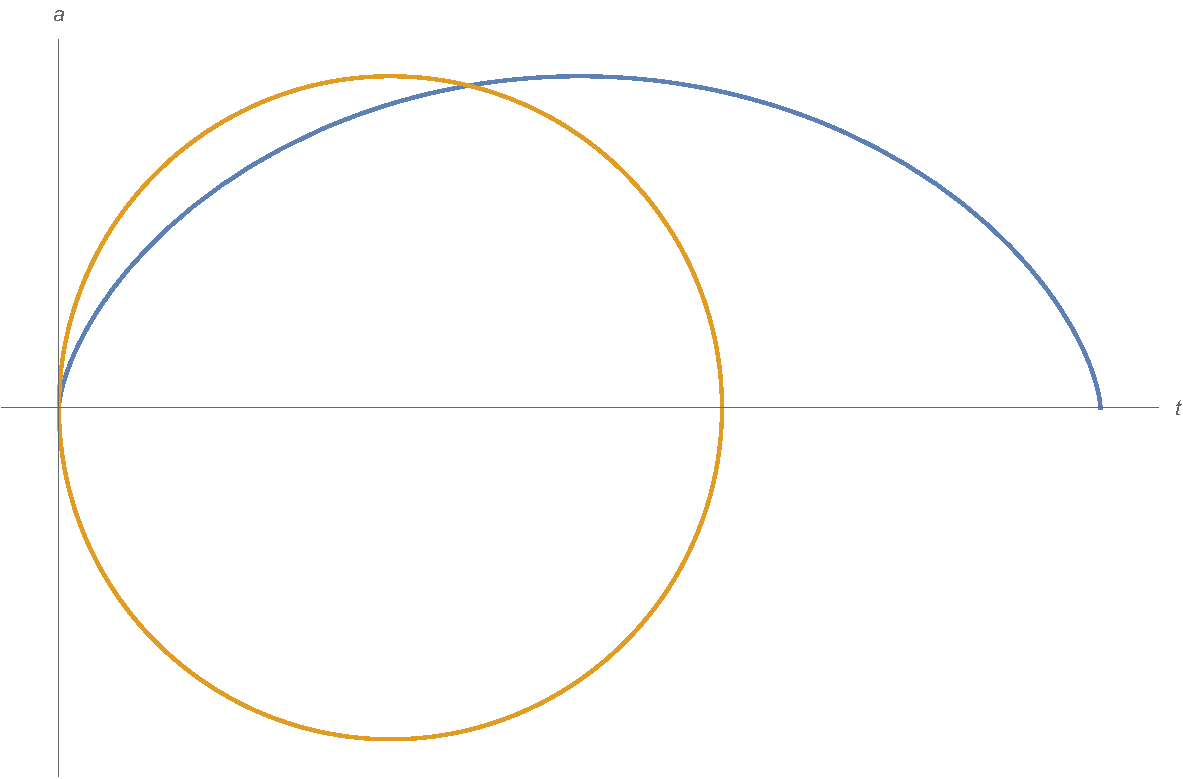
\includegraphics[width=0.7\columnwidth]{parametricPlot.pdf}
        \caption{Parametric plots showing the radius of the dust-filled universe (orange) and
          the radiation-filled universe (blue) versus time}
      \end{figure}
      \newpage
      In the figure, I graphed for $\eta\in[0,2\pi]$ so that when $\eta = 2\pi$
      the dust-filled universe has $a=0$ and when $\eta = \pi$ the
      radiation-filled universe has $a=0$. This means that for a beam of light
      that begins to travel radially at $\psi=0,\eta=0$, the dust-filled
      universe expands and then contracts back to a point exactly when the light
      beam has traveled through all possible $\psi$ values from $0$ to $2\pi$.
      Interestingly, for the radiation-filled universe, we have that the
      expansion and subsequent contraction happens faster so that the light beam
      has only traveled through $\pi$ of the possible $\psi$ values when the
      universe again shrinks back to a point. \\
    \end{solution}
    
    
  \item \textit{Does this mean that one could see the back of one's head in either
      or both of these models?}\\

    \begin{solution}
      No! For the entire lifetime, the particle travels radially. The light beam
      moves at the speed of light but the physical space the light moves through
      is shrinking. To illustrate the effect of this contraction of space we have chosen
      a coordinate system that maps infinity to $\psi=2\pi$ by taking regular
      $\E^3$ and instead writing it as $\mathbb{S}^3$ multiplied by this weird
      $a(\eta)$ factor.\\

      For the radiation-filled universe, we certainly don't see the back of our
      head because by the time the light beam makes it half-way through the
      universe, everything has shrunk to a point for which we no longer have a
      good concept of direction. For the dust-filled universe, we could maybe
      see the back of our head, but again, by the time the light makes it all
      the way around the universe to reach the back of our head, physical space
      has shrunk down to a point and I can no longer talk about direction. It
      seems as though all of the light in the universe must be hitting every
      side of my head at the same time.
    \end{solution}
  \end{enumerate}

\item \textbf{NEW COORDINATES} \\
  Determine functions $f$ and $h$ so that the line element
  \begin{equation}
    ds^2 = -f(\rho)^2dt^2 + h(\rho)^2\Big(d\rho^2 + \rho^2(d\theta^2+\sin^2\theta d\phi^2) \Big)
  \end{equation}
  is (locally) equivalent to the Schwarzschild line element
  \begin{equation}
    ds^2 = -\left( 1-\frac{2m}{r} \right)dt^2 + \frac{dr^2}{1-\frac{2m}{r}}+r^2\Big(d\theta^2+\sin^2\theta d\phi^2 \Big)
  \end{equation}
  \textit{You may assume that $\rho$ only depends on $r$, and that $r>2m$. If you
    integrate by hand, you may find the substitution $r=m(1+\cosh\alpha)$ to be helpful.}\\

  \begin{solution}
    By direct comparison of the two line elements, we can identify the following
    relationships that must hold
    \begin{equation}
      f^2 = 1-\frac{2m}{r} \qquad h^2d\rho^2 = \frac{1}{1-\frac{2m}{r}}dr^2 \qquad h^2\rho^2 = r
    \end{equation}
    If we divide the middle equation by the rightmost equation, we find
    \begin{equation}
      \frac{1}{r^2-2mr}dr^2 = \frac{1}{\rho^2}d\rho^2
    \end{equation}
    which tells us
    \begin{equation}
      \frac{1}{\sqrt{r^2-2mr}} dr = \frac{1}{\rho}d\rho
    \end{equation}
    This is a separable nonlinear ordinary differential equation that we can try
    and integrate to find $r(\rho)$. To aid in this integration, let
    \begin{equation}
      r = m(1+\cosh\alpha)
    \end{equation}
    so that
    \begin{align}
      dr &= m\sinh\alpha\; d\alpha\\
      r^2-2mr &= m^2(1+\cosh^2\alpha+2\cosh\alpha)-2m(1+\cosh\alpha)\\
      &= m^2\left\{ \cosh^2\alpha-1 \right\} = m^2\sinh^2\alpha
    \end{align}
    Therefore, we have
    \begin{align}
      \int \frac{dr}{\sqrt{r^2-2mr}} &= \int \frac{m\sinh\alpha}{\sqrt{m^2\sinh^2\alpha}} \;d\alpha\\
      &= \int d\alpha = \alpha
    \end{align}
    and the other integral is
    \begin{equation}
      \int \frac{d\rho}{\rho} = \ln(\rho)+K
    \end{equation}
    where K is a dimensionful integration constant. In summary, we have found that
    \begin{align}
      \alpha &= \ln(\rho)+K \\
      \Rightarrow r(\rho) &= m(1+\cosh(\ln(\rho)+K)) \\
             &= m\left( 1 + \frac{e^{\ln\rho + K}+e^{-\ln\rho-K}}{2} \right) \\
      &= m\left( 1+\frac{e^K\rho+e^{-K}\frac{1}{\rho}}{2} \right)
    \end{align}
    we will now set the constant $K=0$ for simplicity although this will make it
    impossible to think about dimensions. Thus
    \begin{equation}
      r(\rho) = m\left( 1 + \frac{\rho^2+1}{2\rho} \right) = m\left( \frac{\rho^2+2\rho+1}{2\rho} \right) = m\left( \frac{(\rho+1)^2}{2\rho} \right)
    \end{equation}
    From this expression, we can find the equations for $f(\rho)$ and $h(\rho)$.
    They are
    \begin{align}
      h(\rho) = \frac{r}{\rho} = m\left( \frac{(\rho+1)^2}{2\rho^2} \right)
    \end{align}
    \begin{align}
      f^2(\rho) &= 1-\frac{2m}{r} = 1-\frac{2m}{m\left( \frac{(\rho+1)^2}{2\rho} \right)}  \\
                &= 1-\frac{4\rho}{(\rho+1)^2}\\
      \Rightarrow f(\rho) &= 1-\frac{4\rho}{(\rho+1)^2}
    \end{align}
  \end{solution}

\item \textbf{GODEL GEOMETRY}\\
  The Godel geometry can be described in ``rectangular'' coordinates by the line
  element
  \begin{equation}
    ds^2 = \frac{1}{2\omega^2}\Big( -(dt+e^xdy)^2+dx^2+\frac{1}{2}e^{2x}dy^2+dz^2   \Big)
  \end{equation}
  with $\omega$ constant and $t,x,y,z\in\R$.
  
  \begin{enumerate}[leftmargin=2em, label=(\textbf{\alph*})]
  \item Show that this geometry satisfies Einstein's equation with a perfect
    fluid source.\\
    
    \begin{solution}
      To do this, we will need to calculate the Einstein tensor in order to
      compare it to the stress-energy tensor for the perfect fluid. To do this,
      we can first simplify our calculation by defining an orthonormal basis of
      1-forms from the metric i.e.
      \begin{align}
        \sigma^T &= \frac{1}{\sqrt{2}\omega}(dt+e^xdy) \\
        \sigma^x &= \frac{1}{\sqrt{2}\omega}dx \\
        \sigma^y &= \frac{1}{2\omega}e^x dy \\
        \sigma^z &= \frac{1}{\sqrt{2}\omega}dz
      \end{align}
      in this orthonormal basis of 1-forms, the line element becomes
      \begin{equation}
        ds^2 = -\left(\sigma^T\right)^2+\left( \sigma^x \right)^2+\left( \sigma^y \right)^2+\left( \sigma^z \right)^2
      \end{equation}
      so that the (covariant) metric can be identified as
      \begin{equation}
        (g_{ij}) = \begin{pmatrix} -1 & 0 & 0 & 0 \\ 0 & 1 & 0 & 0 \\ 0 & 0 & 1 & 0 \\ 0 & 0 & 0 & 1 \end{pmatrix}
      \end{equation}

      Using this metric and the above othonormal basis 1-forms, the Ricci
      curvature tensor $R_{ij}$ can be calculated using Tevian's online front
      end to sage differential geometry package. The following shows how I used
      the Kerr geometry demo to calculate the Ricci tensor

      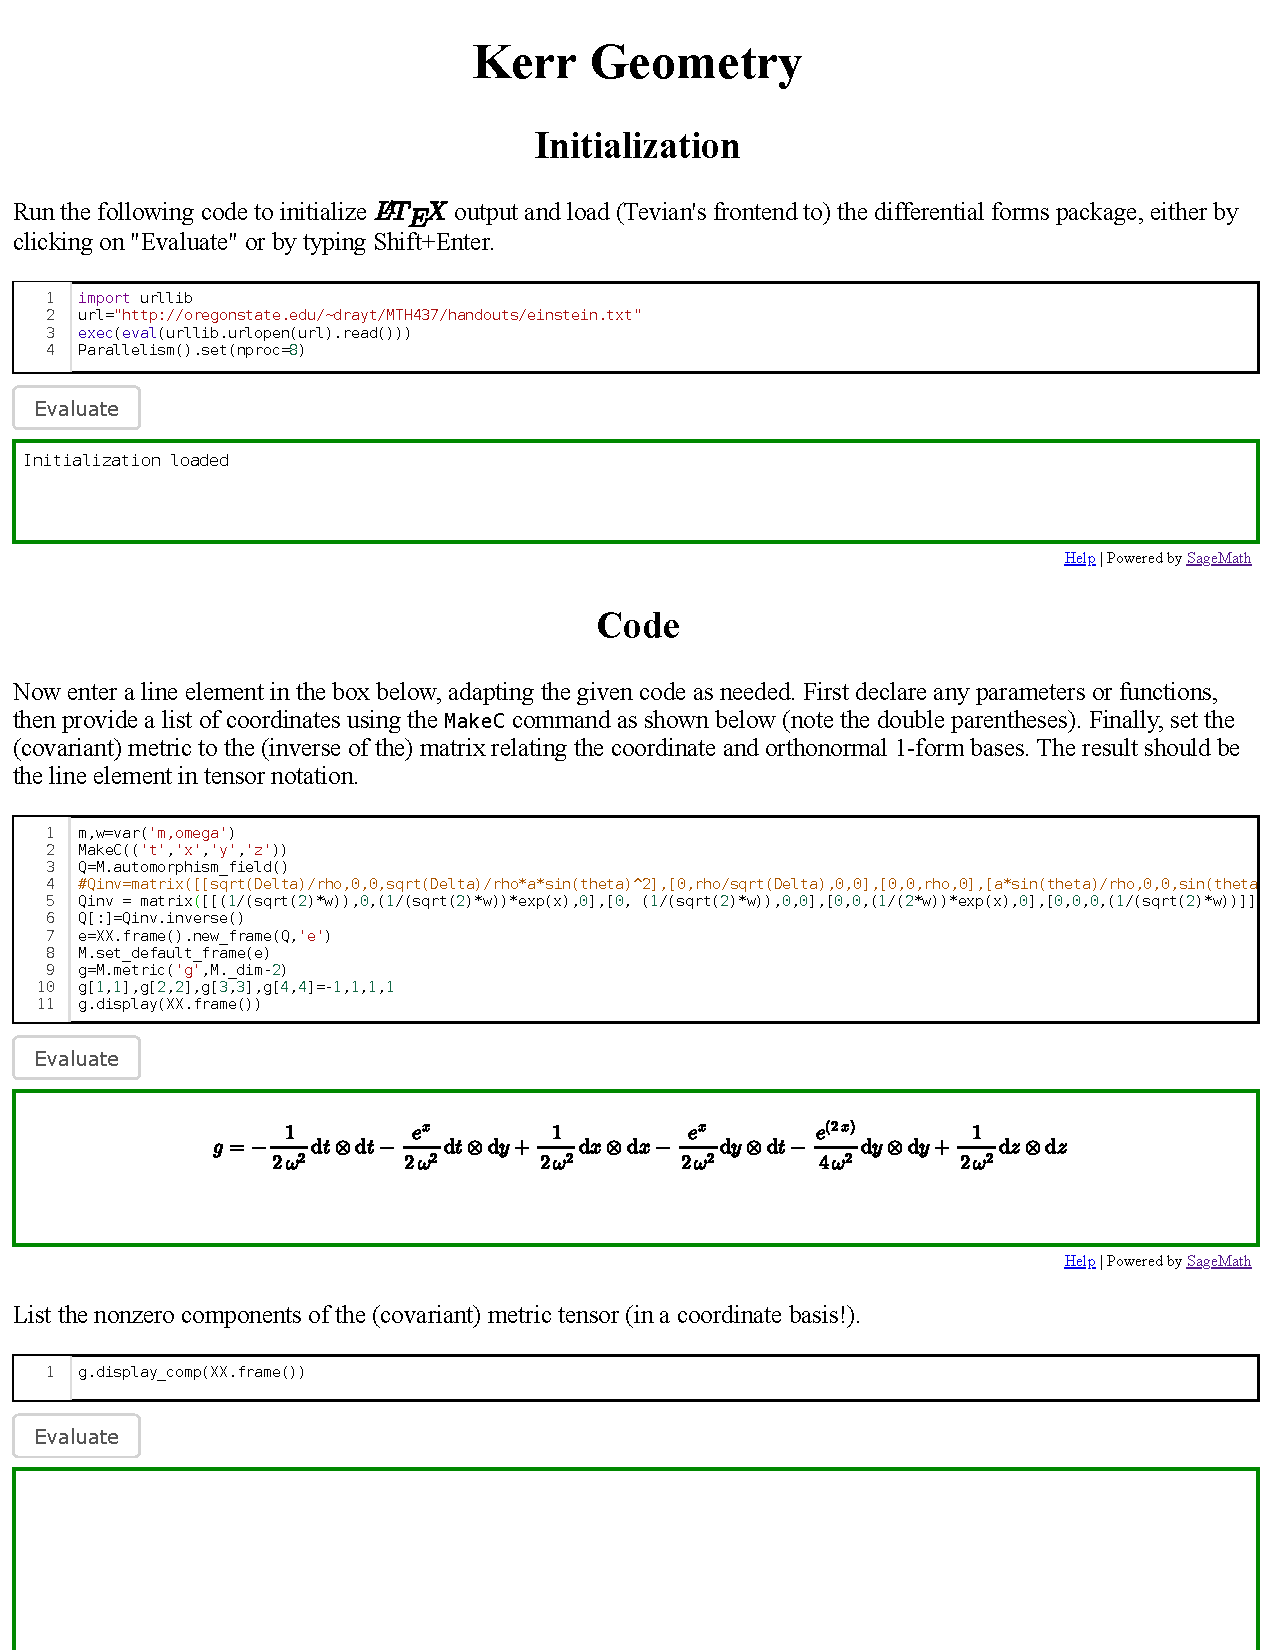
\includepdf[pages=-]{ricciCalc.pdf}


      As we can see from the calculation, the Ricci curvature tensor is
      \begin{equation}
        \left( R_{ij} \right) = \begin{pmatrix}2\omega^2 & 0 & 0 & 0 \\ 0&0&0&0\\ 0&0&0&0\\ 0&0&0&0\end{pmatrix}
      \end{equation}
      The Einstein tensor is defined as
      \begin{equation}
        G_{ij} = R_{ij}-\frac{1}{2}g_{ij}R
      \end{equation}
      where $R$ is the Ricci scalar which for this case is just $R=2\omega^2$.
      Putting this all together, we have
      \begin{equation}
        \left( G_{ij} \right) = \begin{pmatrix} 2\omega^2 & 0 & 0 & 0 \\
          0 & 0 & 0 & 0 \\
          0 & 0 & 0 & 0 \\
          0 & 0 & 0 & 0\end{pmatrix}-\omega^2\begin{pmatrix} -1 & 0 & 0 & 0 \\
          0 & 1 & 0 & 0 \\
          0 & 0 & 1 & 0 \\
          0 & 0 & 0 & 1 \end{pmatrix} = \begin{pmatrix} 3\omega^2 & 0 & 0 & 0 \\
          0 & -\omega^2 & 0 & 0 \\
          0 & 0 & -\omega^2 & 0 \\
          0 & 0 & 0 & -\omega^2\end{pmatrix}
      \end{equation}
      The stress-tensor for a perfect fluid in its rest frame is given by
      \begin{equation}
        (T_{ij}) = \begin{pmatrix} \rho & 0 & 0 & 0 \\
          0 & p & 0 & 0 \\
          0 & 0 & p & 0 \\
          0 & 0 & 0 & p \end{pmatrix}
      \end{equation}
      And therefore, we see that Einstein's equation
      \begin{equation}
        G_{ij}+\Lambda g_{ij} = 8\pi T_{ij}
      \end{equation}
      is satisfied by the above as each of these matrices is diagonal with the
      three spatial components being the same. \\
    \end{solution}
    
  \item What are the allowed values of the cosmological constant $\Lambda$, the
    energy density $\rho$, and the pressure $p$? \textit{Make reasonable
      physical assumptions}.\\

    \begin{solution}
      To decide what the allowed values should be, let's write out the two
      equations that (53) leads to for the perfect fluid. They are
      \begin{align}
        3\omega^2-\Lambda &= 8\pi\rho \\
        -\omega^2+\Lambda &= 8\pi p
      \end{align}
      It is physically reasonable to assume a positive energy density $\rho>0$
      because stuff exists and it's moving around. It is also reasonable to expect
      pressure density to be positive in the sense that gravity is attractive,
      not repulsive... (to be honest, I'm not entirely sure here). However, if we
      do require that $\rho,p > 0$  then it must follow that $\Lambda>0$ because
      $\omega^2>0$. After searching around the internet, I think that taking
      $\Lambda = 2\omega^2$ would lead to an interesting result, namely
      \begin{align}
        \omega^2 &= 8\pi\rho \\
        \omega^2 &= 8\pi p
      \end{align}
      in which case we have that $\rho$ and $p$ are of the same magnitude and
      therefore, the resulting model is neither matter dominated nor radiation dominated.
      I think this is the assumption made on the wikipedia entry found at
      \url{https://en.wikipedia.org/wiki/G%C3%B6del_metric} under ``Einstein Tensor''.\\
    \end{solution}
    
  \item The Godel line element can be ``rewritten'' in cylindrical coordinates as:
    \begin{equation}
      ds^2 = \frac{2}{\omega^2} \Big[ -(dT+\sqrt{2}\sinh^2(r)d\phi)^2 + dr^2+(\sinh^2(r)+\sinh^4(r))d\phi^2+dz^2 \Big]
    \end{equation}
    with $T, r, z\in \R$ and $\phi \in \mathbb{S}$ (the unit circle).
    \textit{You do not need to verify this equivalence!}.
    Consider circles with $T, r,$ and $z$ constant. Are these curves timelike,
    spacelike, or null?\\

    \begin{solution}
      For this case, the line element simplifies to
      \begin{align}
        ds^2 &= \frac{2}{\omega^2}\Big(-2\sinh^4(r)+\sinh^2(r)+\sinh^4(r)   \Big)d\phi^2\\
        &= \frac{2}{\omega^2}\Big( \sinh^2(r)-\sinh^4(r)  \Big)d\phi^2
      \end{align}
      In order to classify these curves, we need to decide if $ds^2>0$, $ds^2<0$
      or $ds^2=0$. For $ds^2$ to be non-trivially zero, we require
      \begin{equation}
        \sinh^2(r) = \sinh^4(r) \quad\Rightarrow\quad 1 = \sinh^2(r)
      \end{equation}
      So solutions to the above equation will tell us the regions where such
      curves are spacelike, null, and timelike. The following graph shows what
      the plot of $1-\sinh^2(r)$ looks like for $r\geq 0$.
      \begin{figure}[!hbt]
        \centering
        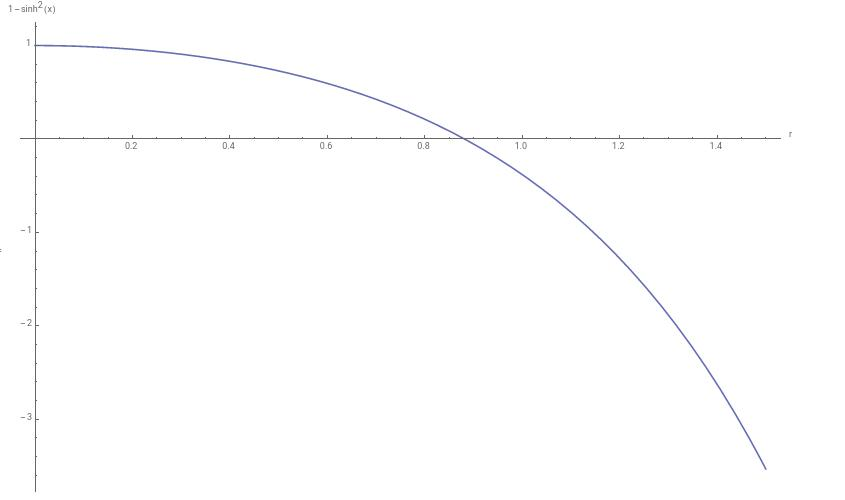
\includegraphics[width=0.5\columnwidth]{godel.jpeg}
      \end{figure}
      There is clearly an inner region for small $r$ where such curves
      are spacelike ($ds^2>0$) one intersection point where the curve is null,
      and then (surprisingly!) curves that are completely timelike! That's
      really weird!\\
    \end{solution}
    
  \item Comment \textit{briefly} on the implications of your result in part
    (c).\\
    
    \begin{solution}
      We just found an infinite number of curves for which traveling in a circle i.e.
      $\phi$ going from $0\to 2\pi$, is completely timelike. That means I just
      found a trajectory through spacetime that allows for travel (without going faster than
      the speed of light) to the past! Apparently such curves are commonly
      called Closed-Timelike-Curves (CTC) and this geometry which contains them
      was an attempt by Godel to show that GR can be inconsistent with reality
      and needs fixing. 
    \end{solution}
    
  \end{enumerate}
\end{enumerate}

\end{document}






























